%% LaTeX2e class for student theses
%% sections/content.tex
%%
%% Karlsruhe University of Applied Sciences
%% Faculty of  Computer Science and Business Information Systems
%%
%% --------------------------------------------------------
%% | Derived from sdqthesis by Erik Burger burger@kit.edu |
%% --------------------------------------------------------

\chapter{Implementation}
\label{ch:Implementation}

\section{Implemented Use Cases}
\label{ch:Implementation:sec:Implemented Use Cases}

Afterwards, the implemented use cases will be described in details.

\subsection{Create Reservation}
\label{ch:Implementation:sec:Implemented Use Cases:ssec:Create Reservation}

\begin{figure}[!ht]
    \centering
    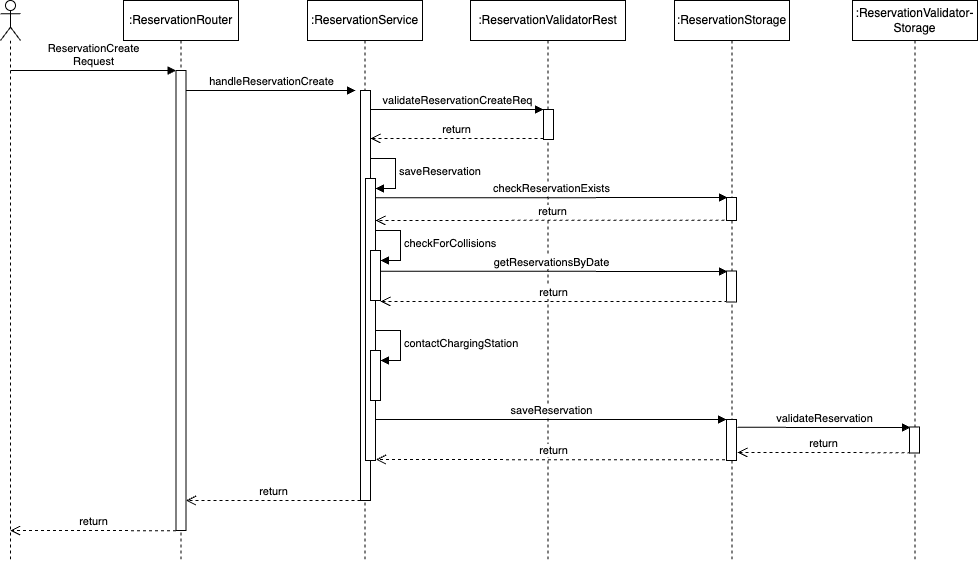
\includegraphics[scale=0.4]{resources/images/main/6_implementation/ReservationCreate.png}
    \caption{Flow of information through the single components of the backend service}
    \label{fig:create-reservation-seq-flow}
\end{figure}

\subsection{Update Reservation}
\label{ch:Implementation:sec:Implemented Use Cases:ssec:Update Reservation}


\begin{figure}[!ht]
    \centering
    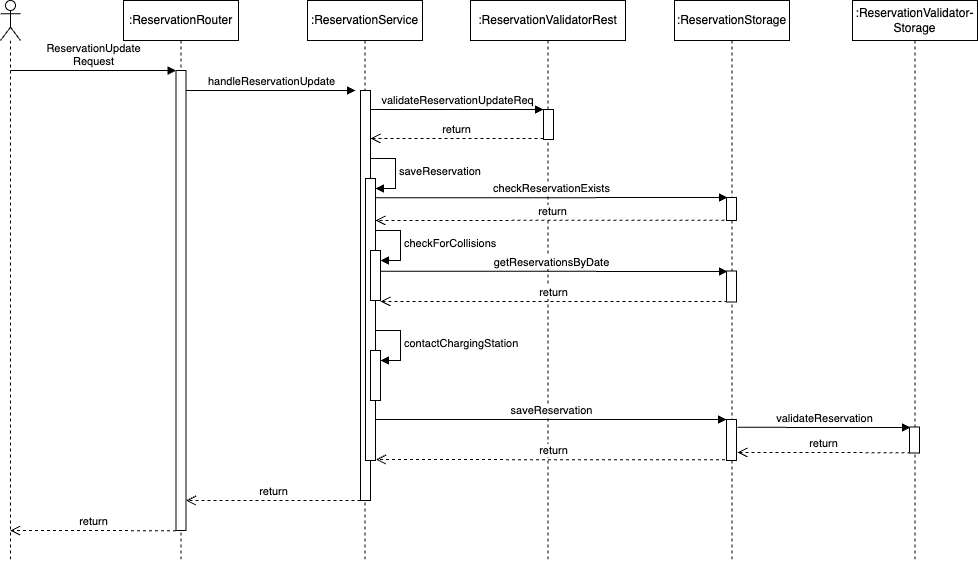
\includegraphics[scale=0.4]{resources/images/main/6_implementation/ReservationUpdate.png}
    \caption{Flow of information through the single components of the backend service}
    \label{fig:update-reservation-seq-flow}
\end{figure}

\subsection{Delete Reservation}
\label{ch:Implementation:sec:Implemented Use Cases:ssec:Delete Reservation}

\begin{figure}[!ht]
    \centering
    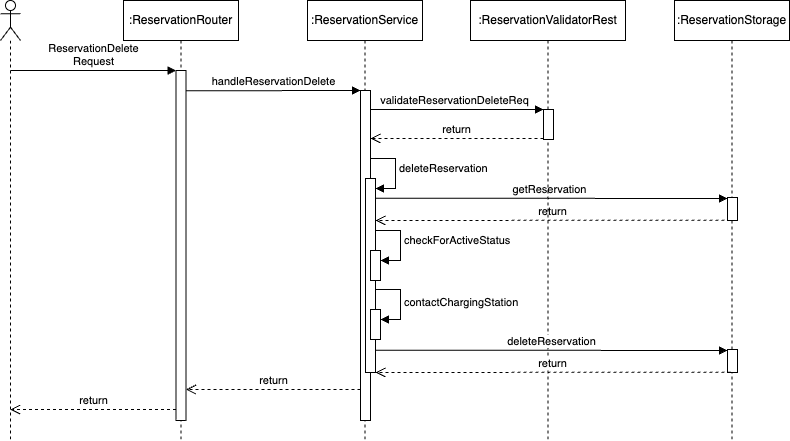
\includegraphics[scale=0.4]{resources/images/main/6_implementation/ReservationDelete.png}
    \caption{Flow of information through the single components of the backend service}
    \label{fig:delete-reservation-seq-flow}
\end{figure}

\subsection{Cancel Reservation}
\label{ch:Implementation:sec:Implemented Use Cases:ssec:Cancel Reservation}


\begin{figure}[!ht]
    \centering
    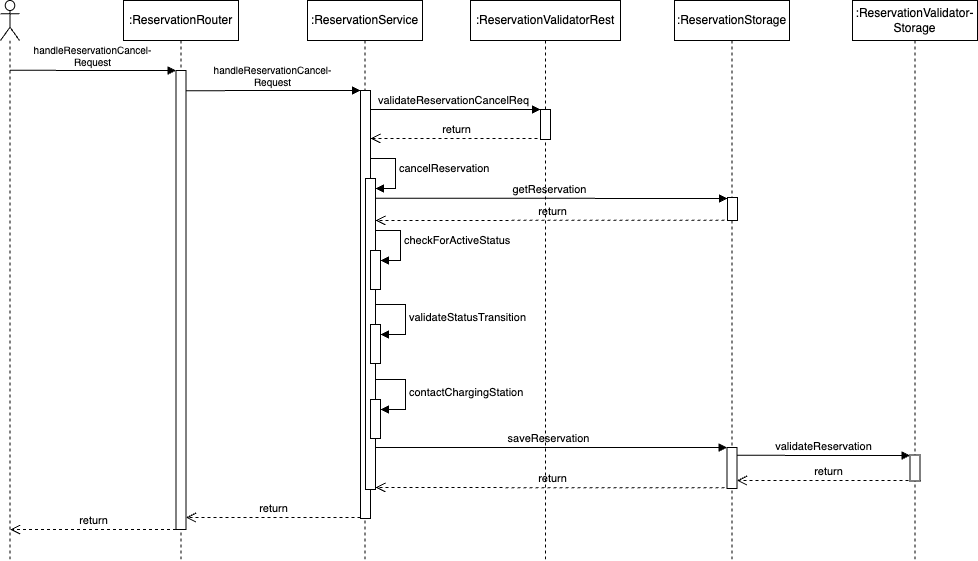
\includegraphics[scale=0.4]{resources/images/main/6_implementation/ReservationCancel.png}
    \caption{Flow of information through the single components of the backend service}
    \label{fig:cancel-reservation-seq-flow}
\end{figure}

\subsection{Schedule Reservation}
\label{ch:Implementation:sec:Implemented Use Cases:ssec:Schedule Reservation}


\begin{figure}[!ht]
    \centering
    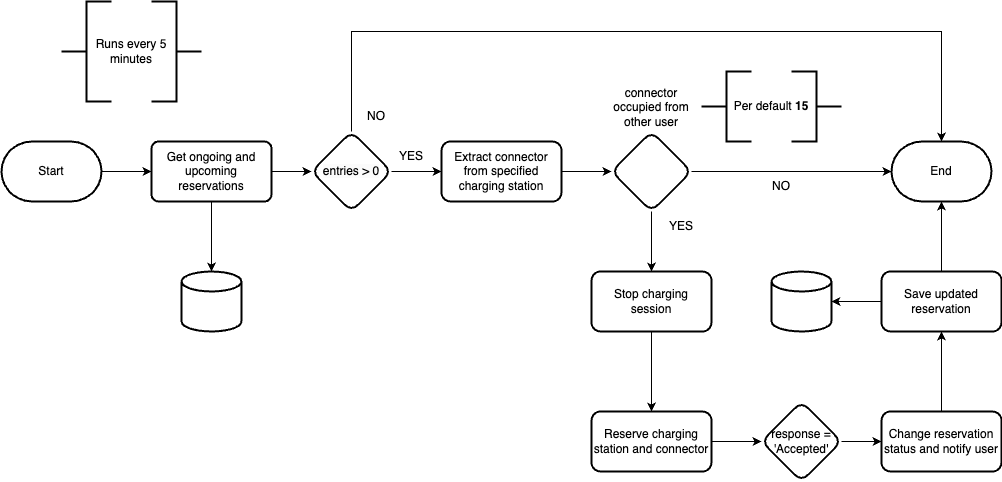
\includegraphics[scale=0.4]{resources/images/main/6_implementation/scheduler/SynchronizeReservation.png}
    \caption{Flow of information through the single components of the backend service}
    \label{fig:schedule-reservation-flow}
\end{figure}

\subsection{Expire Reservation}
\label{ch:Implementation:sec:Implemented Use Cases:ssec:Expire Reservation}

\dots

\subsection{Free reserved connectors}
\label{ch:Implementation:sec:Implemented Use Cases:ssec:Free reserved connectors}

\begin{figure}[!ht]
    \centering
    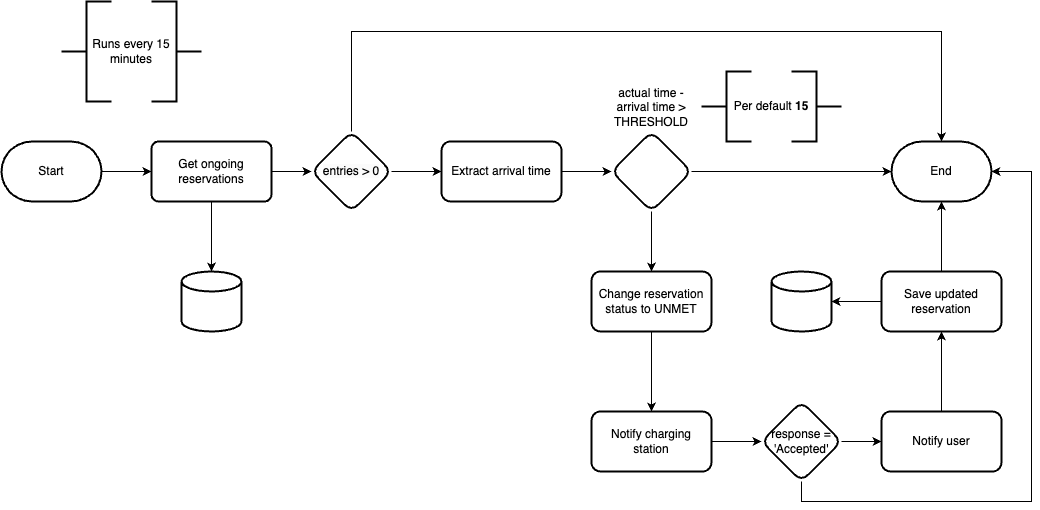
\includegraphics[scale=0.4]{resources/images/main/6_implementation/scheduler/CancelUnmetReservation.png}
    \caption{Flow of information through the single components of the backend service}
    \label{fig:free-connector-flow}
\end{figure}